\chapter*{Lecture 21}
\begin{recall}{}{}
\begin{itemize}
\item MUC the judicious guess
\item MUC and gave examples for:
\begin{itemize}
\item $F(x)$ in the form of an exponential
\item $F(x)$ in the form of a polynomial
\end{itemize}

\end{itemize}
\end{recall}






\section*{4.5 Method of Undetermined Coefficients (MUC)}
Here is a helpful table to remove some of the guess work:
\begin{figure}[h!]
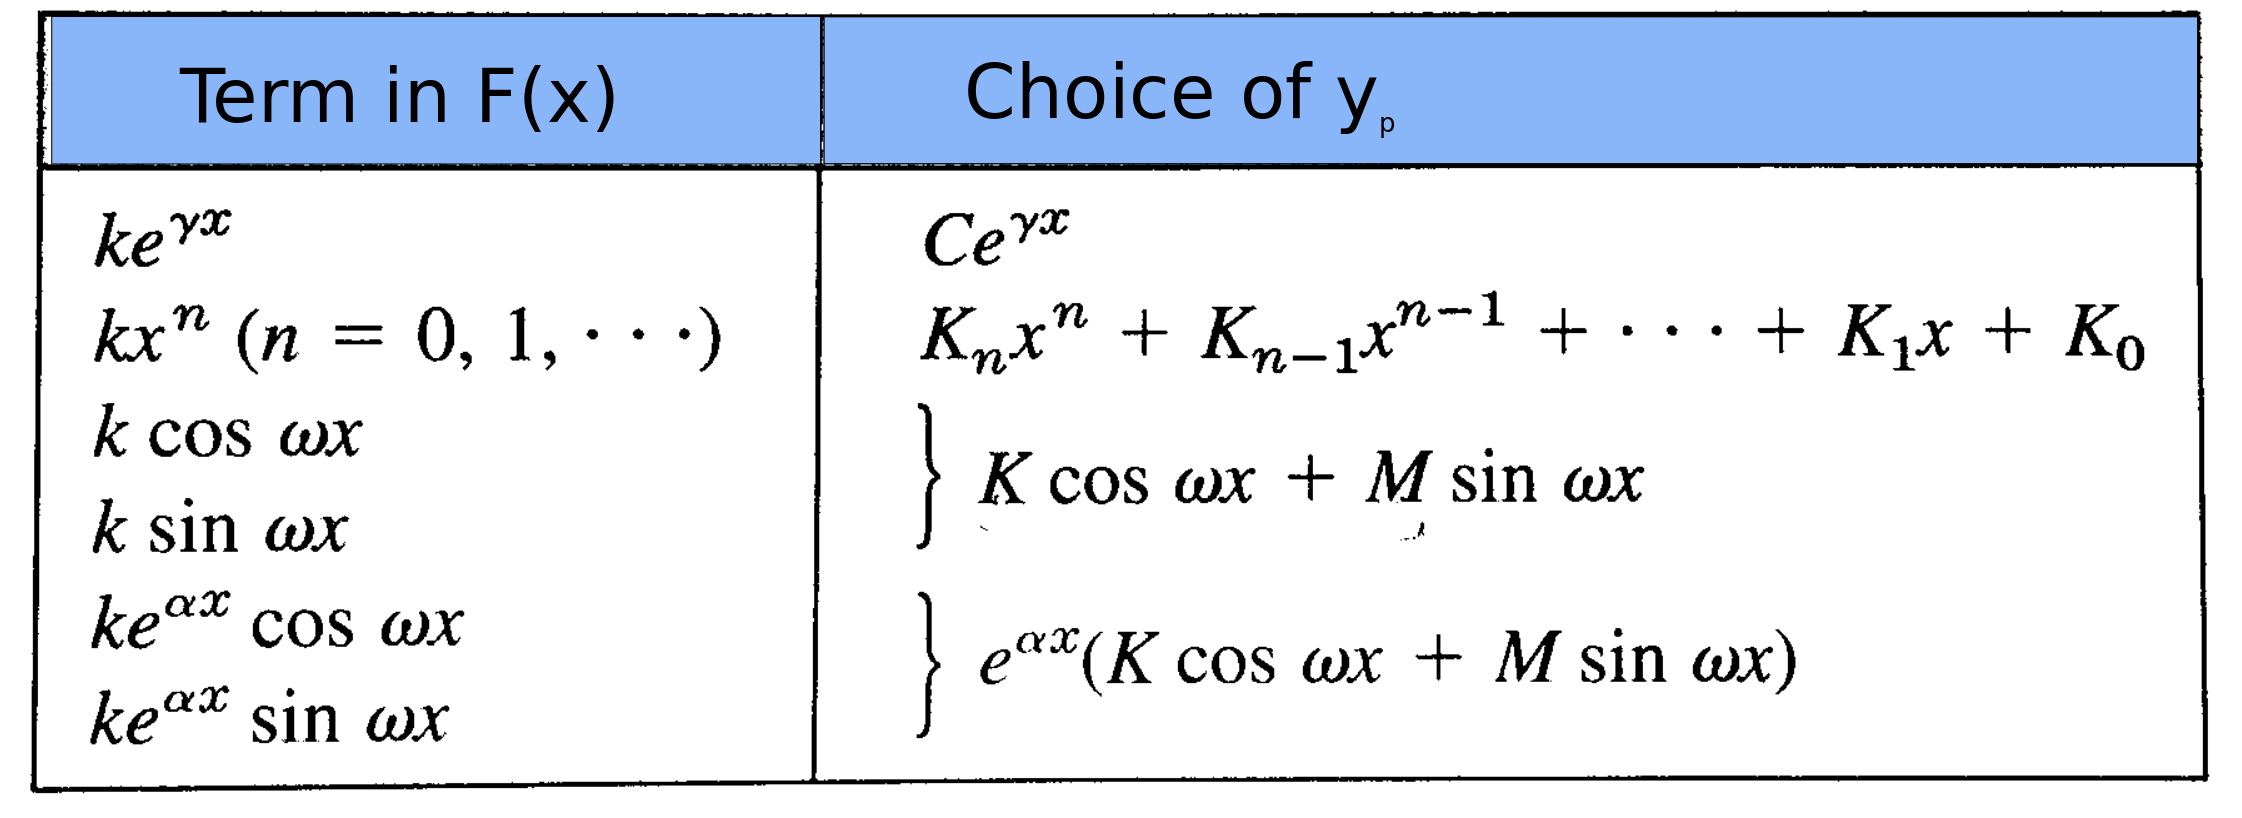
\includegraphics[width=\textwidth]{figs/MUC_2.png} 
\end{figure}
We will add new entries to this table as we move along. This table is meant to help, and does not always provide us the form of $y_p$!


\begin{exmp}{MUC:}\\
Solve the following non-homogeneous equation:
\begin{equation*}
y''-3y'-4y=2\sin(x)
\end{equation*}
Solution:\\

\begin{equation}
y_{g}=y_{h} + y_{p} 
\end{equation}
\begin{itemize}
\item Homogeneous solution:
(same as previous example!)
\begin{align*}
y_h=C_1 e^{4x}+C_2 e^{-x}\\
\end{align*}
\item Particular solution:
We guess that our solution looks something like: $y_p=A\sin(x)+B\cos(x)$\\
\begin{align*}
y'_p=A\cos(x)-B\sin(x) \qquad  y''_p=-A\sin(x)-B\cos(x)
\end{align*}

We sub into our ODE:
\begin{equation*}
(-A\sin(x)-B\cos(x))-3(A\cos(x)-B\sin(x))-4(A\sin(x)+B\cos(x))=2\sin(x)
\end{equation*}
We sum all the sines and cosines on the RHS:
\begin{equation*}
(-5A+3B)\sin(x)+(-3A-5B)\cos(x))=2\sin(x) + (0\cos(x))
\end{equation*}
A system of equation with 2 equations and 2 unknowns:
\begin{align*}
(-5A+3B)=2\\
(-3A-5B)=0
\end{align*}
Can solve by multiplying the top equation by 5 and the bottom by 3 and adding them together:
\begin{align*}
(-25A+15B)=10\\
(-9A-15B)=0\\
-34A=10 \qquad or \qquad A=-10/34
\end{align*}
We find $B=3/17$

\begin{align*}
y_p=-10/34\sin(x)+3/17\cos(x)
\end{align*}
\end{itemize}
The general solution is then:
\begin{align*}
y_{general}=y_h+y_p=C_1 e^{4x}+C_2 e^{-x} -10/34\sin(x)+3/17\cos(x)
\end{align*}
\end{exmp}



\begin{exmp}{MUC (superposition):}\\
Solve the following non-homogeneous equation:
\begin{equation*}
y''-3y'-4y=2\sin(x)+3e^{2x}
\end{equation*}
Solution:\\
What do we do now????\\
Let's recall the previous examples:
\begin{itemize}
\item $y''-3y'-4y=0$ (homogeneous)
\begin{align*}
y_h=C_1 e^{4x}+C_2 e^{-x}
\end{align*}
\item $y''-3y'-4y=3e^{2x}$ (particular - last lecture)
\begin{align*}
y_{p_1}=- \frac{e^{2x}}{2}
\end{align*}
\item $y''-3y'-4y=2\sin(x)$ (particular - this lecture)
\begin{align*}
y_{p_2}=-10/34\sin(x)+3/17\cos(x)
\end{align*}
\end{itemize}
The general solution is then:
\begin{align*}
y_g=y_h+y_{p_1}+y_{p_2}=C_1 e^{4x}+C_2 e^{-x} - \frac{e^{2x}}{2}-10/34\sin(x)+3/17\cos(x)
\end{align*}
\end{exmp}

Let's raise the level a bit more!

\begin{exmp}{MUC:}\\
Solve the following non-homogeneous equation:
\begin{equation*}
4y''-4y'+y=9xe^{2x}
\end{equation*}
[This is a combination of an exponential and polynomial forcing term]
Solution:
\begin{itemize}
\item Find the homogeneous solution:\\
Aux Eq: $4r^2-4r+1=0$ gives the following root: $r_1=r_2=1/2$\\
The solution is: $y_1=e^{x/2}$ and $y_2=xe^{x/2}$
\begin{equation*}
\boxed{y_h=C_1 e^{x/2} + C_2xe^{x/2}}
\end{equation*}
\item Find the particular solution:\\
We assume a solution of the form: $y_p=(ax+b)e^{2x}$, we can derive this solution such that:
\begin{align*}
y'_p=ae^{2x}+2(ax+b)e^{2x}=(2ax+a+2b)e^{2x}\\
y''_p=2ae^{2x}+2(2ax+a+2b)e^{2x}= (4ax+4a+4b)e^{2x}
\end{align*}
Sub into the ODE:
\begin{equation*}
4(4ax+4a+4b)e^{2x}-4(2ax+a+2b)e^{2x}+(ax+b)e^{2x}=9xe^{2x}
\end{equation*}

simplification...
\begin{align*}
4(4ax+4a+4b)-4(2ax+a+2b)+(ax+b)=9x\\
9ax +12 a+ 9b = 9ax
\end{align*}
\begin{align*}
9a=9 \qquad 12a+9b=0\\
a = 1 \qquad b =-4/3
\end{align*}


\begin{align*}
\boxed{y_p = (x-\frac{4}{3})e^{2x}}
\end{align*}
\item General solution:
\begin{align*}
\boxed{y_g =C_1 e^{x/2} + C_2xe^{x/2}+ (x-\frac{4}{3})e^{2x}}
\end{align*}
\end{itemize}
\end{exmp}


